\subsection{Operating Principles}
\label{subsec:Actuators, Operating Principles}
Despite the variability in fluidic elastomer actuator morphologies, their fundamental operating principles are universal.
This section provides an overview of these operating principles.
Generally, each segment of a fluidic elastomer robot bends and this bending is due to material strain.
Figure~\ref{fig:ElastomerBending} illustrates how unidirectional bending arises from material strain.
Consider a block of elastomer where the edges of the top and bottom surfaces have equal lengths, $L_0$.
If the top surface is strained such that its new edge length is $L_0$ + $\Delta L$, but the bottom of this block remains unextended, then the elastomer will bend.
Bending is the basic motion primitive of the fluidic elastomer robot.
\begin{figure}[htb]
\centering
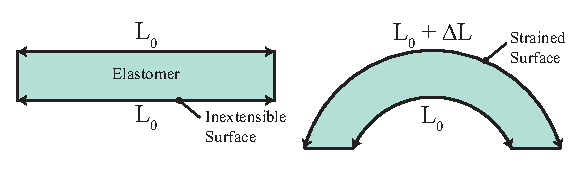
\includegraphics[width=0.85\columnwidth]{figures/actuators/ElastomerBending.eps}
\caption[Operating principle of a bending elastomer segment.]{Operating principle of a bending elastomer segment. One surface of the elastomer is strained while the opposite side remains unextended. The difference in length produces bending.}
\label{fig:ElastomerBending}
\end{figure}

In order to generate strain within the elastomer, this class of actuator uses pressurized fluids.
Essentially, expandable, fluid-filled chambers are embedded within the elastomer.
When these chambers are pressurized, the entrapped fluid generates stress in the material causing the material to strain.
This concept is illustrated in Figure~\ref{fig:FluidicPower}A and Figure~\ref{fig:FluidicPower}B.
Here, the entrapped fluid is shown in yellow and its pressure is $p_c$.
In order to express the relationship between fluid pressure and elastomer deformation, we can use a one-dimensional simplification of an iterative model presented in \citet{marchese2015design}.
Let $\bar{h}$ and $\bar{t}$ be the initial undeformed diameter and wall thickness of a cylindrical elastomer channel, and let $\hat{h}$ and $\hat{t}$ represent the deformed diameter and wall thickness.
Algorithm~\ref{alg:SimpleModel} expresses how the channel's diameter grows as a function of pressure.
Stresses are successively updated based on deformed channel dimensions.
Here, $\Delta \mathbf{p}_{c}$ is a vector of all consecutive incremental pressure increases until the maximum channel pressure $p_c^{\text{max}}$ is reached.
The stress and strain in the elastomer are represented by $\sigma$ and $\epsilon$, respectively.
The procedure \texttt{strainLookUp()} provides a nonlinear mapping from stress to strain.
\begin{algorithm}[htb]
\footnotesize
  \DontPrintSemicolon
  \SetAlgoLined
  \caption{Iterative Channel Deformation}
  \label{alg:SimpleModel}
  \KwIn{$\bar{t}$, $\bar{h}$, $\Delta \mathbf{p}_{c}$, $p_c^{\text{max}}$}
  $\hat{h} \gets \bar{h}$. \;
  $\hat{t} \gets \bar{t}$. \;
  $\bar{c} \gets \pi \, \left(\frac{\bar{t}}{2} + \bar{h} + \frac{\bar{t}}{2}\right)$. \;
  $p_c \gets p_{\text{atm}}$. \;
  $i \gets 0$. \;
  \Repeat{$p_c \geq p_c^{\text{max}}$}
  {
     $\sigma \gets p_c \frac{\hat{h}}{2 \,\hat{t}}$. \;
     $\epsilon \gets \texttt{strainLookUp}(\sigma)$. \;
     $\hat{c} \gets \bar{c}\left( 1 + \epsilon \right)$. \;
     $\hat{h}, \hat{t} \gets \texttt{solve}\left\{
	\begin{array}{l}
       \text{\textbf{Circumferential Strain:}} \\
       \hat{h} = \frac{\hat{c}}{\pi} - \hat{t} \\
       \text{\textbf{Conservation of Material Volume:}} \\
       \pi \left[ \left( \frac{\hat{h}}{2} + \hat{t}\right)^2 - \frac{\hat{h}^2}{4} \right]= \pi \left[\left( \frac{\bar{h}}{2} + \bar{t}\right)^2 - \frac{\bar{h}^2}{4}\right]
     \end{array}
     \right\} $. \;
     $p_c \gets p_c + \Delta p_{c,i}$. \;
     $i++$
   }
\normalsize
\end{algorithm}

\begin{figure}[htb]
\centering
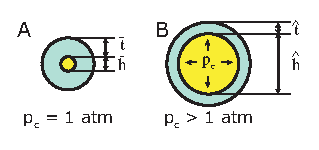
\includegraphics[width=2.0in]{figures/actuators/FluidicPower.eps}
\caption[Operative principle of producing material strain through fluidic power.]{Operative principle of producing material strain through fluidic power. (\textbf{A}) Fluid, shown in yellow, is entrapped in an elastomer channel. (\textbf{B}) When the fluid is pressurized, stress and therefore strain are generated in the material. }\label{fig:FluidicPower}
\end{figure}
